\documentclass[12pt, french]{report}

\usepackage[top=3cm, bottom=3cm, left=3cm, right=3cm]{geometry}
\usepackage[T1]{fontenc}
\usepackage[utf8]{inputenc}
\usepackage{babel}
\usepackage{graphicx}
\usepackage{hyperref}
\usepackage{pdfpages}
\usepackage{gensymb}
\usepackage{eurosym}
\usepackage{xcolor}
\usepackage{appendix}
\usepackage{amsmath,amsfonts,amssymb}

\hypersetup{                    % parametrage des hyperliens
    colorlinks=true,                % colorise les liens
    breaklinks=true,                % permet les retours à la ligne pour les liens trop longs
    urlcolor= blue,                 % couleur des hyperliens
    linkcolor= blue,                % couleur des liens internes aux documents (index, figures, tableaux, equations,...)
    citecolor= green                % couleur des liens vers les references bibliographiques
    }
   
\begin{titlepage}
\title{	
\includegraphics[scale=0.4]{assets/img/logo-adaltas.png}\\[1 cm]
		\normalsize \textsc{Rapport de stage}\\[0.8cm]
		{Entreprise partenaire : \\Adaltas}\\[0.8 cm]
		{Representée par :\\David Worms - david@adaltas.com}\\[0.5 cm]
		\rule{\linewidth}{0.2 mm} \\[0.4 cm]
		\LARGE \textbf{\uppercase{Mise en place d'une solution d'automatisation et de déploiement pour NodeJS}}
		\rule{\linewidth}{0.2 mm}
		}
\author {\normalsize Auteur :\\	\normalsize Alexander Hoffmann - alexander@adaltas.com\\[0.5 cm]
		 \normalsize Mentor :\\	\normalsize David Worms - david@adaltas.com\\}
\date{\normalsize \today}
\end{titlepage}

\begin{document}
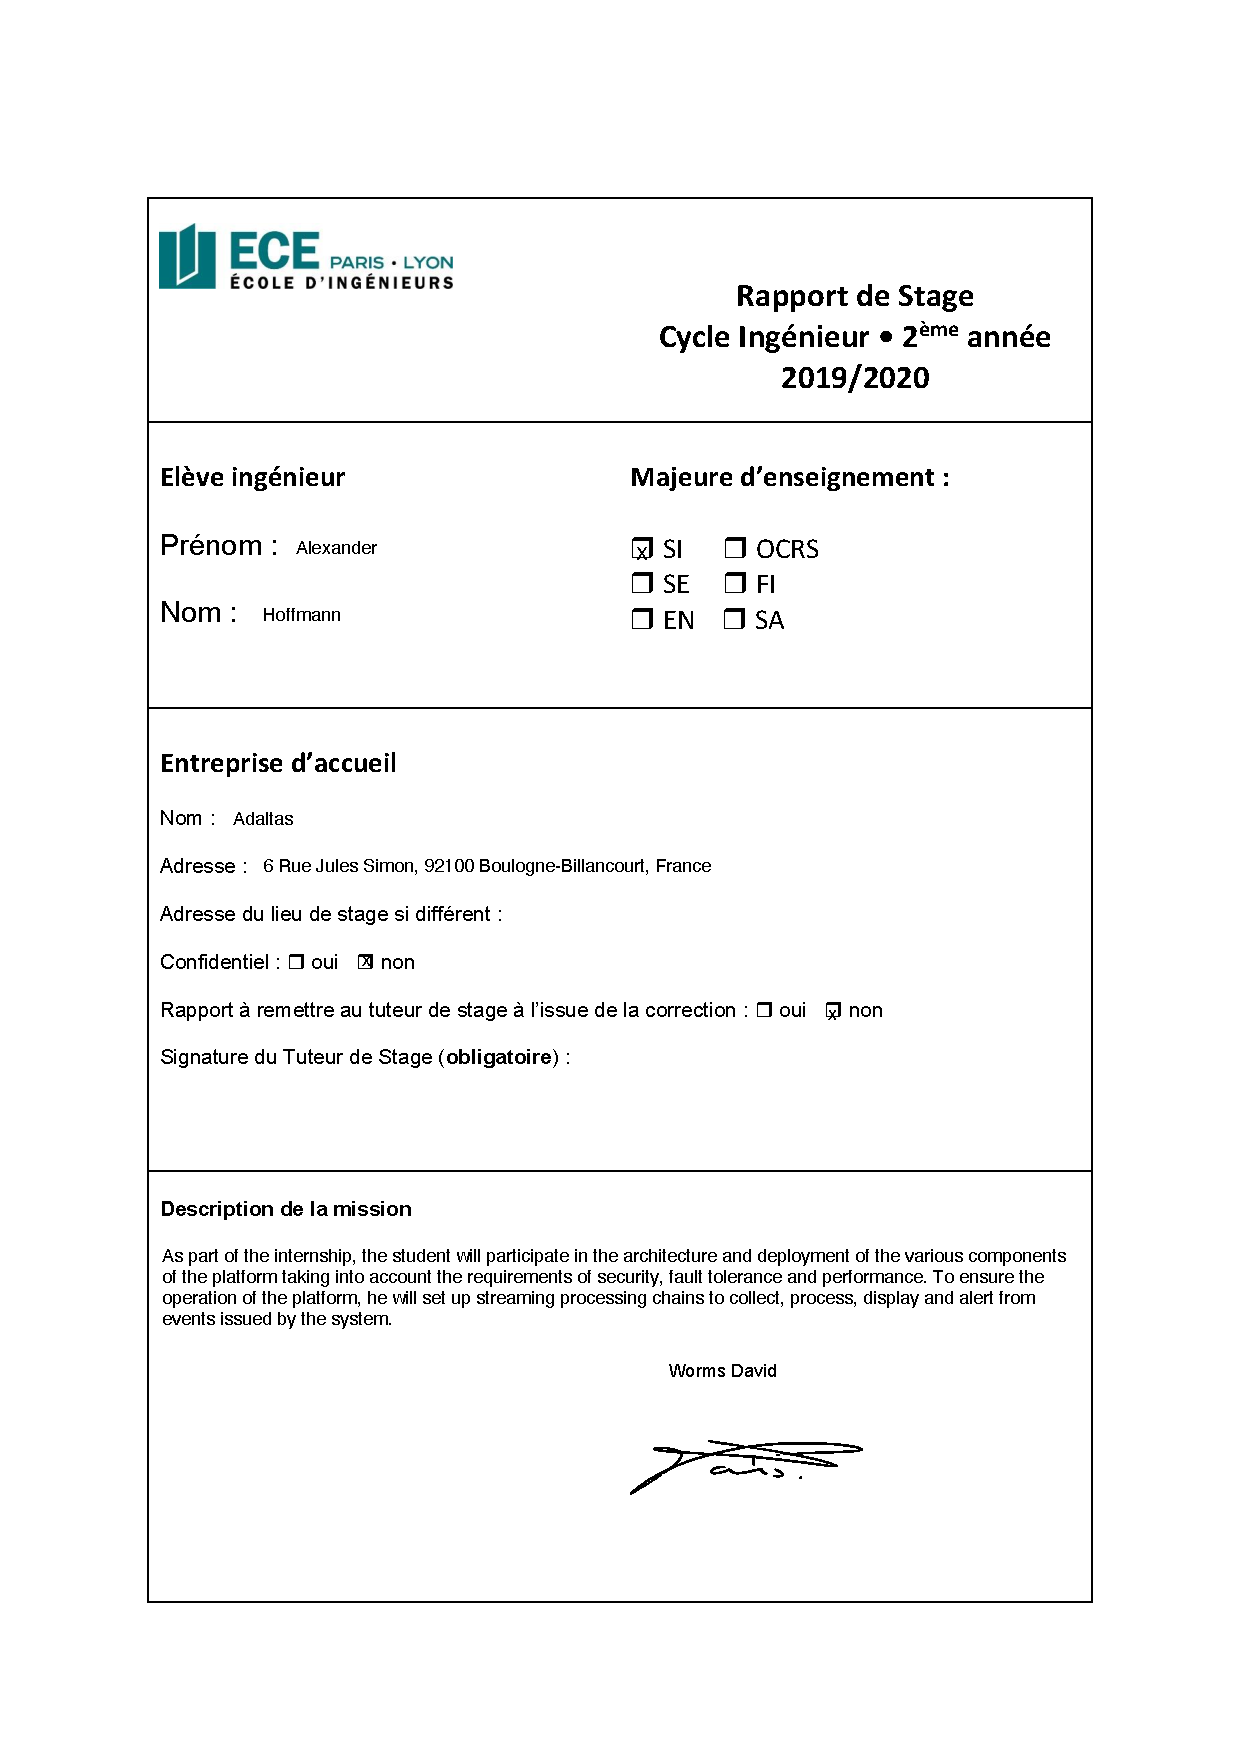
\includepdf[pages=-]{assets/pdf/title.pdf}

\maketitle

\begingroup
\hypersetup{linkcolor=black}
\tableofcontents
\listoffigures
\newpage
\endgroup

\chapter*{Remerciements}

Je tiens tout d’abord à remercier toute l'équipe d'Adaltas pour son accueil, sa disponibilité et sa bonne
humeur permanente.\\

Je voudrais ensuite exprimer ma sincère gratitude à David Worms, mon tuteur, pour la confiance qu’il a bien voulu m’accorder en acceptant de m'intégrer à Adaltas. Je le remercie pour sa grande disponibilité, sa patience, son soutien chaleureux et ses conseils avisés. Je tiens à lui exprimer ma profonde reconnaissance pour ses critiques constructives d’une rigueur absolue.\\

Mes remerciements s’adressent également à Prisca Borges pour son accueil, sa sympathie et ses conseils, ainsi qu'à Léo Schoukroun pour son encadrement et sa compréhension qu'il m'a accordé tout au long du stage.

\end{document}
